% B.Tech. project report (Report 2): EEG-based multi-neurodevelopmental disorder detection with
% SMVMD common modes and Riemannian geometry.
% Built on the IIT Indore BTP template. Every number comes from generated/r2_numbers.tex and
% generated/final_numbers.tex (and generated/tab_*.tex), written by report/build_report2.py and
% report/build_final.py from results/. Do not type numbers here.
%
%   python report/build_final.py ; python report/build_report2.py      (from the repo root)
%   cd report/report2 && pdflatex BTP_report2 && pdflatex BTP_report2
%
\documentclass[12pt, a4paper, oneside]{report}
% ---- FILL IN THESE SIX LINES; they are used on the title page, declaration,
% ---- preface, certificate and acknowledgements.
\newcommand{\StudentName}{[Student Name]}
\newcommand{\RollNo}{[Roll No.]}
\newcommand{\SupervisorName}{[Prof.\ Supervisor Name]}
\newcommand{\SupervisorDetails}{[designation, Department of Electrical Engineering]}
\newcommand{\SubmissionMonth}{[Month]}
\newcommand{\SubmissionYear}{2026}
\usepackage{fancyhdr}
\linespread{1.5}
\usepackage{cite}
\usepackage[T1]{fontenc}
\usepackage{lmodern}
\usepackage{geometry}
\usepackage{amsmath,amssymb,amsthm}
\usepackage{graphicx}
\usepackage{float}
\usepackage{array}
\usepackage{setspace}
\usepackage{hhline}
\usepackage{booktabs}
\usepackage{adjustbox}
\usepackage{enumitem}
\usepackage{tikz}
\usetikzlibrary{arrows.meta,positioning}
\usepackage[hidelinks]{hyperref}
\geometry{verbose,a4paper,tmargin=15mm,bmargin=22mm,lmargin=30mm,rmargin=20mm}
\renewcommand\bibname{References}
\DeclareGraphicsExtensions{.pdf,.png,.jpeg}
\graphicspath{{figures/}}

% ---- generated numbers: \R{Name} prints the value, or ?? if it is not yet computed
\InputIfFileExists{generated/final_numbers.tex}{}{\typeout{*** run report/build_final.py first ***}}
\InputIfFileExists{generated/r2_numbers.tex}{}{\typeout{*** run report/build_report2.py first ***}}
\newcommand{\R}[1]{\ifcsname #1\endcsname\csname #1\endcsname\else\textbf{??}\fi}
\newcommand{\gentable}[1]{\IfFileExists{generated/#1.tex}{\begin{adjustbox}{max width=\textwidth}\input{generated/#1.tex}\end{adjustbox}}{\textbf{[#1 not yet generated]}}}
\newcommand{\genfig}[2][0.9\textwidth]{%
  \IfFileExists{figures/#2.pdf}{\includegraphics[width=#1]{#2}}{\fbox{\parbox{0.8\textwidth}{\centering figure #2 not yet generated}}}}
\newcommand{\dstwonote}{$^\ast$DS-2: the ADHD children were on methylphenidate (Ritalin) and controls were not, so any ADHD-vs-control difference may reflect medication rather than ADHD.}

\begin{document}
\begin{titlepage}
\setstretch{1.15}
\begin{center}
\vspace*{10pt}
{\LARGE \bf EEG-Based Multi-Neurodevelopmental\\[4pt] Disorder Detection using\\[4pt]
 SMVMD Common Modes and Riemannian Geometry} \\
\vspace{20pt}
{\large \bf B.Tech.\ Project }\\
\vspace{20pt}
\emph{Submitted in partial fulfillment of the requirements \\of the degree of}\\[4pt]
{\large \bf Bachelor of Technology} \\
{\large in}\\
{\large \bf Electrical Engineering}\\
\vspace{20pt}
By \\[4pt]
{\large \bf \StudentName} \\
(Roll No.\ \RollNo)\\
\vspace{14pt}
Under the guidance of\\[4pt]
{\large \bf \SupervisorName}\\
\vspace{20pt}

\includegraphics[height=4.0cm]{IITI.png}\\
\vspace{16pt}
{\Large \bf Department of Electrical Engineering \\[2pt]
 Indian Institute of Technology Indore \\[2pt]
 \SubmissionMonth\ \SubmissionYear}
\end{center}
\end{titlepage}

\pagenumbering{roman}
\setcounter{page}{1}

% Declaration, preface, certificate, acknowledgements, abstract. Names come from the fill-in
% block at the top of BTP_report2.tex.
\newpage
\begin{center}{\Large\bf Declaration}\end{center}
\par I hereby declare that the project entitled ``EEG-Based Multi-Neurodevelopmental Disorder
Detection using SMVMD Common Modes and Riemannian Geometry'' submitted in partial fulfillment for
the award of the degree of Bachelor of Technology in Electrical Engineering completed under the
supervision of \SupervisorName, \SupervisorDetails, IIT Indore is an authentic work.
\par Further, I declare that I have not submitted this work for the award of any other degree elsewhere.
\par I declare that this written submission represents my ideas in my own words and where
others' ideas or words have been included, I have adequately cited and referenced the original
sources. I also declare that I have adhered to all principles of academic honesty and integrity
and have not misrepresented or fabricated or falsified any idea/data/fact/source in my submission.
I understand that any violation of the above will be cause for disciplinary action by the
institute and can also evoke penal action from the sources which have thus not been properly
cited or from whom proper permission has not been taken when needed.
\vspace{2cm}
\begin{flushright}\StudentName\\ Roll No.\ \RollNo\end{flushright}
\begin{flushleft}Date: ........................\\ Place: ........................\end{flushleft}

\newpage
\begin{center}{\Large\bf Preface}\end{center}
This report on \textbf{``EEG-Based Multi-Neurodevelopmental Disorder Detection using SMVMD
Common Modes and Riemannian Geometry''} is prepared under the guidance of \SupervisorName.

The project addresses the detection of two neurodevelopmental disorders, intellectual and
developmental disorder (IDD) and attention-deficit/hyperactivity disorder (ADHD), from
electroencephalogram (EEG) recordings with one common framework. Its central result is a
lightweight pipeline that combines an adaptive multichannel decomposition with the Riemannian
geometry of channel covariance matrices and gradient-boosted trees, evaluated strictly on people
the model has never seen. Every number in this report is generated by code from saved result
files.
\vspace{2cm}
\begin{flushleft}\StudentName\\ B.\ Tech.\ IV year\\ Department of Electrical Engineering\end{flushleft}

\newpage
\begin{center}{\Large\bf B.\ Tech.\ Project Approval Certificate}\vspace{1.0cm}\end{center}
\par This is to certify that the dissertation titled \textbf{``EEG-Based
Multi-Neurodevelopmental Disorder Detection using SMVMD Common Modes and Riemannian Geometry''}
submitted by \textbf{\StudentName} (Roll No.\ \RollNo) is approved for the award of
degree of \textbf{Bachelor of Technology} in \textbf{Electrical Engineering.}
\vspace{1.0cm}
\begin{flushright}
BTP Supervisor: \hspace{0.7cm} \SupervisorName\\[0.8cm]
Signature: \hspace{0.7cm} ......................................\\ \vspace{1.0cm}
Date: \hspace{0.7cm} ......................................\\ \vspace{1.0cm}
Designation: \hspace{0.7cm} ......................................\\
\end{flushright}

\newpage
\begin{center}{\Large\bf Acknowledgements}\end{center}
% DRAFT: personalise before submission.
\par I am grateful to my supervisor, \SupervisorName, for guidance and encouragement throughout
this project, and in particular for the suggestion to combine the mode decomposition with the
Riemannian approach, which became the main pipeline of this work.
\par I thank the Department of Electrical Engineering, IIT Indore, for the facilities and
support provided during my B.Tech.\ studies.
\par I thank the authors of the two public EEG datasets used in this work, and the participants
and families who contributed recordings to them.
\par Finally, I thank my family and friends for their constant support.
\vspace{1.5cm}
\begin{flushright}\StudentName\end{flushright}

\newpage
\begin{center}{\Large\bf Abstract}\end{center}
Neurodevelopmental disorders are diagnosed from behaviour, which is slow and depends on
specialist judgement. This project develops an EEG-based framework that detects two such
disorders, intellectual and developmental disorder (IDD) and attention-deficit/hyperactivity
disorder (ADHD), with the same processing for both, on two public datasets: 14 participants
recorded at rest and during music (IDD) and 121 children recorded during a visual attention task
(ADHD).

Accuracies of 95--100\% are reported for both datasets in the literature, but most of them are
obtained by dividing the short windows of each person between the training and test sets, or do
not report keeping people apart. Re-implemented in this work, the best-reported method classifies
\R{DStwoSegWinAcc}\% of ADHD windows correctly when windows are split in this way, but only
\R{DStwoSubjWinAcc}\% when the test children are unseen. Every result here is therefore obtained
with subject-wise cross-validation, nested tuning on training subjects only and majority voting
per person.

The proposed pipeline decomposes every window with successive multivariate variational mode
decomposition (SMVMD), groups the window-specific modes into four common modes ($\delta$,
$\theta$, $\alpha$, $\beta$) by their centre frequencies, represents each common mode by its
channel covariance matrix, maps the matrices to the Riemannian tangent space and classifies with
gradient-boosted trees (LightGBM). On unseen ADHD children it reaches \R{MainDStwoBal}\%
balanced accuracy (AUC \R{MainDStwoAUC}) and classifies
\R{MainDStwoSubj} children correctly; on IDD it classifies all participants correctly in all three
recording settings. The ADHD result is comparable to the best published subject-wise result on the same
data, obtained with a deep convolutional network, while the proposed pipeline needs no GPU, takes
about \R{RtTotal}~ms of single-core computation per 5-second window and trains in about
\R{RtTrain}~s. Ablations show that the channel covariance in the tangent space carries the
information, that LightGBM gives the highest scores on it, and that the adaptive decomposition
does not by itself add accuracy over fixed band-pass filtering. The ADHD
children were medicated and the controls were not, which limits the interpretation of all ADHD
results. The work is a research study and not a diagnostic tool.

\vspace{2mm}
\noindent\textbf{\emph{Keywords}} -- EEG, ADHD, intellectual and developmental disorder,
variational mode decomposition, Riemannian geometry, gradient boosting, subject-independent
evaluation, data leakage.


\tableofcontents
\listoffigures
\addcontentsline{toc}{chapter}{List of Figures}
\listoftables
\addcontentsline{toc}{chapter}{List of Tables}

\chapter*{List of Abbreviations}
\addcontentsline{toc}{chapter}{List of Abbreviations}
\begin{tabbing}
xxxxxxxxxxxx \= \kill
ADHD \> Attention-deficit/hyperactivity disorder\\
ADMM \> Alternating direction method of multipliers\\
AUC \> Area under the ROC curve\\
CI \> Confidence interval (95\%, percentile bootstrap over subjects)\\
CNN \> Convolutional neural network\\
CV \> Cross-validation\\
EEG \> Electroencephalography\\
GBDT \> Gradient-boosted decision trees\\
IDD \> Intellectual and developmental disorder\\
KNN \> $k$-nearest neighbours\\
LOSO \> Leave-one-subject-out cross-validation\\
LR \> Logistic regression\\
LSTM \> Long short-term memory network\\
mRMR \> Minimum redundancy maximum relevance\\
NC \> Normal controls (DS-2)\\
OAS \> Oracle approximating shrinkage (covariance estimator)\\
ROC \> Receiver operating characteristic\\
SPD \> Symmetric positive definite (matrix)\\
(S)(M)VMD \> (Successive) (multivariate) variational mode decomposition\\
SVM \> Support vector machine\\
TDC \> Typically developing controls (DS-1)\\
\end{tabbing}

\newpage
\pagenumbering{arabic}
\setcounter{page}{1}
\chapter{Introduction}
\thispagestyle{empty}

\section{Background}
Neurodevelopmental disorders are conditions that begin in the developmental period and affect
personal, social, academic or occupational functioning~\cite{apa2013}. Two of them are studied
in this project. Attention-deficit/hyperactivity disorder (ADHD) is characterised by
inattention, hyperactivity and impulsivity; a pooled estimate of its worldwide prevalence in
children and adolescents is about 5\%~\cite{polanczyk2007}. Intellectual and developmental
disorder (IDD), also called intellectual disability, combines significantly below-average
intellectual functioning with limitations in adaptive behaviour; its prevalence is about
1\%~\cite{maulik2011}.

Both disorders are diagnosed from behaviour: clinical interviews, rating scales completed by
parents and teachers, and standardised tests, interpreted by a specialist according to criteria
such as DSM-5~\cite{apa2013}. The process is slow, depends on the availability of specialists
and involves subjective judgement. An objective physiological measurement that supports the
diagnosis would therefore be valuable.

Electroencephalography (EEG) records the electrical activity of the brain from electrodes on
the scalp. It is non-invasive, inexpensive compared with other brain-imaging methods, portable
and has millisecond time resolution, and consumer-grade wireless headsets make recordings
possible outside the hospital. These properties make EEG the most practical candidate for a
physiological aid to the assessment of neurodevelopmental disorders.

\section{Problem statement}
The problem addressed is the \textbf{detection of multiple neurodevelopmental disorders from
EEG}: given an EEG recording, decide whether it comes from a person with the disorder or from a
control, for IDD and for ADHD, with one common processing and classification framework.

Two requirements follow from the intended use. The framework should handle more than one
disorder with the same processing, rather than a method tuned separately for each condition. And
it must work on a person whose EEG it has never seen, because that is the only situation in
which a detection system is used. The second requirement decides how every result in this
report is obtained.

\section{Motivation for the proposed pipeline}
Published methods report accuracies of 95--100\% on the two public datasets used here
(Chapter~2), but most of them divide the short windows of each person between the training and
the test set, or do not report keeping people apart, so that the classifier may be tested on
people it has already seen. When the
method with the highest reported accuracy was re-evaluated on unseen people in this project, its
accuracy fell to little above chance (Chapter~4). A broad comparison of alternatives under a
strict protocol (Chapter~5) then showed that representing each window by the
\emph{covariance matrix of its channels}, analysed with Riemannian geometry, carried the most
information about ADHD. The proposed pipeline (Chapter~6) builds on this finding: it keeps the
adaptive multichannel decomposition (SMVMD) of the starting method to split the signal into
frequency-specific common modes, describes each mode by its channel covariance, and classifies
the Riemannian tangent-space features with gradient-boosted trees.

\section{Objectives}
\begin{enumerate}
\item to develop an EEG classification pipeline that applies unchanged to IDD and ADHD and is
      light enough to run on an ordinary computer without a GPU;
\item to evaluate it on people not seen during training, with a protocol that excludes every
      form of information leakage;
\item to analyse each component of the pipeline (decomposition, common modes, Riemannian
      representation, classifier) by ablation, and to compare the result with published work;
\item to establish what the pipeline relies on, which modes and electrodes carry the
      information, and which properties of the data other than the disorder could explain the
      results.
\end{enumerate}

\section{Contributions}
\begin{itemize}
\item \textbf{A pipeline combining SMVMD common modes, Riemannian geometry and gradient
      boosting.} The window-specific SMVMD modes are mapped to four common modes by centre
      frequency, so that a fixed set of covariance matrices describes every window. On unseen
      ADHD children it reaches \R{MainDStwoBal}\% balanced accuracy and \R{MainDStwoSubj}
      children correct; on IDD all participants are classified correctly.
\item \textbf{A strict evaluation} with subject-wise cross-validation, nested tuning on
      training subjects only, an automated leakage test and majority voting per person.
\item \textbf{Ablations} of the classifier (LR, SVM, XGBoost, LightGBM), of the individual
      modes, and of the decomposition itself against fixed band-pass filters and the undecomposed
      signal.
\item \textbf{A quantified comparison with the literature}, showing how window-level splitting
      inflates reported accuracy, and that the proposed pipeline is comparable with the best
      published subject-wise ADHD result without a deep network or a GPU.
\end{itemize}

\section{Organisation of the report}
Chapter~2 reviews EEG-based detection of ADHD and IDD and the limitations of published
evaluations. Chapter~3 describes the datasets and their preprocessing, and Chapter~4 the
evaluation protocol. Chapter~5 summarises the preliminary study that led to the proposed
pipeline. Chapter~6 describes the pipeline in detail, and Chapter~7 presents its results,
ablations and analyses. Chapter~8 gives the conclusions, limitations and future work.

\chapter{Literature Review}
\thispagestyle{empty}

\section{EEG and its frequency bands}
The EEG is the potential difference between scalp electrodes produced by the summed synchronous
activity of large groups of cortical neurons, with amplitudes of tens of microvolts. Electrodes
are placed according to the international 10--20 system: the letter gives the region (F frontal,
C central, T temporal, P parietal, O occipital), odd numbers lie over the left hemisphere, even
numbers over the right and ``z'' on the midline. Activity is conventionally described in the
delta (1--4~Hz), theta (4--8~Hz), alpha (8--13~Hz), beta (13--30~Hz) and gamma ($>$30~Hz) bands.
The recorded signal also contains non-cerebral contributions: eye movements produce large slow
deflections at frontal electrodes, muscle activity produces broadband activity in the beta and
gamma range, and mains interference appears at 50~Hz. A classifier uses any consistent
difference between groups, whatever its origin, so these contributions matter for detection.

\section{EEG findings in ADHD and IDD}
The most studied EEG finding in ADHD is increased theta and decreased beta power, summarised as
a raised theta/beta ratio~\cite{snyder2006}. A later meta-analysis found that the effect has
become smaller in more recent studies and cannot serve as a reliable diagnostic
measure~\cite{arns2013}. Stimulant medication shifts the EEG of children with ADHD towards that
of controls, mainly in the theta and beta bands~\cite{clarke2002}, so medication status must be
considered whenever ADHD and control groups are compared. EEG studies of intellectual disability
are fewer and the available recordings are small; the dataset used here~\cite{sareen2020data} was
published to support such work.

\section{Methods used for EEG classification}
\textbf{Adaptive decomposition.} EEG is non-stationary and contains several oscillatory
components at once. Empirical mode decomposition~\cite{huang1998} splits a signal into intrinsic
mode functions by an iterative algorithm; variational mode decomposition (VMD)~\cite{dragomiretskiy2014}
replaces the algorithm by an optimisation problem that finds $K$ band-limited modes; multivariate
VMD (MVMD)~\cite{rehman2019} extends it to several channels with centre frequencies shared by all
channels; and successive MVMD (SMVMD)~\cite{liu2022} extracts the modes one after another, so
that their number adapts to each signal.

\textbf{Hand-crafted features} include band powers from the power spectral
density~\cite{welch1967}, Hjorth parameters~\cite{hjorth1970}, entropies~\cite{richman2000,
bandt2002} and connectivity measures between channels such as the weighted phase-lag
index~\cite{vinck2011}. They are classified with $k$-nearest neighbours, support vector
machines~\cite{cortes1995}, random forests~\cite{breiman2001} or gradient-boosted
trees~\cite{chen2016, ke2017}.

\textbf{Riemannian methods} represent a window by the covariance matrix of its channels. These
matrices are symmetric positive definite and lie on a curved manifold; projecting them onto the
tangent space at their mean gives vectors that standard classifiers can
use~\cite{barachant2012, congedo2017}. Riemannian methods were developed for brain--computer
interfaces~\cite{congedo2017}; none of the studies on the two datasets reviewed below uses them.

\textbf{Deep learning} learns features from the raw signal, with compact convolutional networks
such as EEGNet~\cite{lawhern2018} and ShallowConvNet~\cite{schirrmeister2017}, recurrent networks
(LSTM) or hybrids of both~\cite{roy2019}.

\section{Published results on the two datasets}
Table~\ref{tab:lit} lists representative published results on the two datasets used in this
work, with the evaluation protocol \emph{as described by the authors}. Chandela
\emph{et al.}~\cite{chandela2025} detect both disorders with one method: SMVMD of each window,
nine statistical features per mode integrated with an energy weighting, mRMR feature
selection~\cite{peng2005} and $k$-nearest neighbours, with 10-fold cross-validation over windows.
Their accuracies of \R{PaperDSoneAcc}\% (IDD) and \R{PaperDStwoAcc}\% (ADHD) are the highest
reported for a single method covering both datasets, and this method is the starting point of the
present work. Several other ADHD studies on the same dataset report 99\% or more with channel
selection and $k$-NN~\cite{maheshwari2025}, a residual network with attention~\cite{bansal2025} or
CatBoost on a selected feature subset~\cite{mao2025}.

\begin{table}[H]
\caption{Published results on the two datasets, with the evaluation protocol as described in
each paper. ``Window-level'' means that the folds or the train/test split are formed from
windows or samples, so that data of the same person can appear in training and test; a
``not reported'' entry means that the paper does not state that subjects were kept apart.}
\label{tab:lit}\centering\small
\begin{adjustbox}{max width=\textwidth}
\begin{tabular}{p{3.3cm}p{1.2cm}p{4.4cm}p{3.9cm}r}
\hline
Study & Data & Method & Evaluation (as described) & Accuracy (\%) \\
\hline
Chandela \emph{et al.} 2025~\cite{chandela2025} & IDD & SMVMD features, mRMR, KNN & 10-fold over windows & \R{PaperDSoneAcc} \\
Chandela \emph{et al.} 2025~\cite{chandela2025} & ADHD & SMVMD features, mRMR, KNN & 10-fold over windows & \R{PaperDStwoAcc} \\
Maheshwari \emph{et al.} 2025~\cite{maheshwari2025} & ADHD & entropy-based channel selection, KNN & 10-fold / 70:30 split; subject separation not reported & 99.29 \\
Bansal \emph{et al.} 2025~\cite{bansal2025} & ADHD & autoencoder + ResNet with attention & 80:20 split of samples & 99.42 \\
Mao \emph{et al.} 2025~\cite{mao2025} & ADHD & CatBoost, 206 selected features & random 10-fold; subject separation not reported & 99.58 \\
\hline
Geethapriya and Pattabiraman 2026~\cite{geethapriya2026} & ADHD & SVM on spectral features & 10-fold over windows & 90.0 \\
 & & SVM on spectral features & \textbf{subject-wise} 10-fold & 65.6 \\
 & & LSTM & subject-wise 10-fold & 61.6 \\
 & & CNN--BiLSTM & subject-wise 10-fold & 65.7 \\
 & & CNN (their best) & subject-wise 10-fold & 72.7 \\
\hline
\end{tabular}
\end{adjustbox}
\end{table}

\section{Limitations of published evaluations}
\label{sec:leakage}
\textbf{Window-level splitting.} A recording is cut into many short, overlapping windows, and
the windows of one person share everything that is specific to that person and that recording:
head shape, electrode contact, artefacts and individual rhythms. If the folds are formed from
windows, the test windows of a person have near-identical neighbours in the training set, and a
classifier can score highly by recognising the person rather than the disorder. Saeb
\emph{et al.}~\cite{saeb2017} showed for clinical machine learning in general that such
record-wise evaluation overestimates the accuracy on new people, and Brookshire
\emph{et al.}~\cite{brookshire2024} found that most published deep-learning studies of
translational EEG are affected. For the ADHD dataset used here, Geethapriya and
Pattabiraman~\cite{geethapriya2026} measured the effect directly: the same SVM on spectral
features reaches 90.0\% with window-level folds and 65.6\% with subject-wise folds
(Table~\ref{tab:lit}). This project found the same for the starting method (Chapter~4): its
accuracy on ADHD windows falls from \R{DStwoSegWinAcc}\% to \R{DStwoSubjWinAcc}\% when the
children in the test set are new.

\textbf{Small samples.} With 14 participants (IDD) or 121 children (ADHD), cross-validation
estimates are uncertain by several percentage points~\cite{varoquaux2018}, so small differences
between methods are not meaningful.

\textbf{Heavy models.} The best subject-wise ADHD result found in the literature, 72.7\%, was
obtained with a convolutional network trained end to end~\cite{geethapriya2026}, and several of
the other studies use deep or recurrent networks. Such models are usually trained on a GPU and
are hard to interpret, which matters for a clinical aid and for deployment on simple hardware.

\textbf{Confounds.} In the ADHD dataset the children with ADHD were taking methylphenidate and
the controls were not (Chapter~3); published studies rarely discuss this, although stimulants
change the EEG~\cite{clarke2002}.

\section{Research gap}
None of the studies on these datasets reviewed here combines (i) a strict subject-wise
evaluation, (ii) one pipeline for both disorders, and (iii) a lightweight, interpretable model, and no subject-wise result on the IDD dataset was found. This project addresses
these points: it evaluates every method on unseen people, and proposes a pipeline built from
an adaptive decomposition, the Riemannian geometry of channel covariances and gradient-boosted
trees, which runs on a laptop CPU.

\chapter{Datasets and Preprocessing}
\thispagestyle{empty}

Two public datasets are used, one per disorder. They are referred to as DS-1 (IDD) and DS-2
(ADHD). Table~\ref{tab:datasets} summarises them.

\begin{table}[H]
\caption{The two datasets. Window counts are for 5~s windows with 50\% overlap.}
\label{tab:datasets}\centering\small
\begin{tabular}{lp{5.3cm}p{5.3cm}}
\hline
 & DS-1 (IDD)~\cite{sareen2020data} & DS-2 (ADHD)~\cite{motie2020} \\
\hline
Participants & 7 with IDD, 7 typically developing controls (TDC) & 61 with ADHD, 60 normal controls (NC) \\
Age & IDD group \R{DSoneIddAgeMin}--\R{DSoneIddAgeMax} years; controls not given in the dataset files & 7--12 years \\
Device & EMOTIV EPOC+, 14 channels & 19 channels, 10--20 system \\
Sampling rate & 128~Hz & 128~Hz \\
Recording & 2~min rest and 2~min listening to music & visual attention task, length depends on the child \\
Windows & \R{DSoneRestNWin} per condition (\R{DSoneRestWinPerSubjMin} per recording) & \R{DStwoNWin} (\R{DStwoNWinDis} ADHD, \R{DStwoNWinCtrl} NC) \\
Windows per subject & \R{DSoneRestWinPerSubjMin} & \R{DStwoWinPerSubjMin}--\R{DStwoWinPerSubjMax} \\
\hline
\end{tabular}
\end{table}

\section{DS-1: intellectual and developmental disorder}
DS-1~\cite{sareen2020data} contains recordings of 14 participants, 7 with IDD and 7 typically
developing controls, made with a 14-channel EMOTIV EPOC+ headset at 128~Hz. The electrodes are
AF3, F7, F3, FC5, T7, P7, O1, O2, P8, T8, FC6, F4, F8 and AF4. Each participant was recorded
for two minutes at rest and for two minutes while listening to music. The dataset provides both
the raw recordings and cleaned recordings; the cleaned recordings were produced by the dataset
authors in EEGLAB with a 1--30~Hz band-pass filter, removal of line noise, independent component
analysis and automatic rejection of artefact components.

The two recording conditions give three classification settings, all with the same
participants: rest only, music only, and rest and music together. Each recording gives
\R{DSoneRestWinPerSubjMin} windows, so the rest and music settings have \R{DSoneRestNWin}
windows each (\R{DSoneRestNWinDis} IDD and \R{DSoneRestNWinCtrl} TDC) and the combined setting
has \R{DSoneRestMusicNWin}.

\textbf{The participants of DS-1 are adults.} The metadata file distributed with the dataset
gives the ages of the seven IDD participants as \R{DSoneIddAgeMin}--\R{DSoneIddAgeMax} years; it
gives no ages for the controls. The IDD results of this project therefore concern adults, and
only the ADHD results concern children. In this report the terms ``child-level'' and
``subject-level'' are used interchangeably for quantities computed per person; for DS-1 the
person is an adult participant.

\section{DS-2: attention-deficit/hyperactivity disorder}
DS-2~\cite{motie2020} contains recordings of 121 children aged 7--12 years, 61 with ADHD and 60
controls, boys and girls. According to the dataset description reproduced
in~\cite{chandela2025}, ADHD was diagnosed by an experienced psychiatrist using DSM-IV criteria,
and the control children had no history of psychiatric disorders, epilepsy or high-risk
behaviour. EEG was recorded from 19 electrodes of the 10--20 system (Fp1, Fp2, F3, F4, C3, C4,
P3, P4, O1, O2, F7, F8, T3, T4, T5, T6, Fz, Cz, Pz) at 128~Hz. T3, T4, T5 and T6 are the older
names of the positions now called T7, T8, P7 and P8.

The recording protocol was a visual attention task: the child was shown pictures of cartoon
characters and asked to count them, with between 5 and 16 characters per picture. Each picture
was shown until the child answered, so the length of a recording depends on the child's
performance. DS-2 gives \R{DStwoNWin} windows, \R{DStwoNWinDis} from ADHD children and
\R{DStwoNWinCtrl} from controls, with between \R{DStwoWinPerSubjMin} and \R{DStwoWinPerSubjMax}
windows per child.

\textbf{Medication.} The children with ADHD had been taking methylphenidate (Ritalin) for up to
six months; the control children were not medicated. Since stimulant medication changes the
EEG~\cite{clarke2002}, \emph{every ADHD result in this report is a comparison of medicated
children with ADHD against unmedicated controls}, and a classifier may detect the effect of the
drug rather than the disorder. This caveat is repeated wherever ADHD results appear.

\section{Preprocessing}
\textbf{DS-1.} The cleaned recordings distributed with the dataset are used as they are. The
original cleaning used MATLAB toolboxes that have no exact Python equivalent, so using the
distributed cleaned data is the closest match to earlier work on this dataset.

\textbf{DS-2.} The recordings are filtered with a fourth-order Butterworth band-pass filter
(0.5--60~Hz) and a 50~Hz notch filter, both applied forwards and backwards so that no phase
shift is introduced. They are then processed with the discrete wavelet transform, using the
Coiflet-3 wavelet at decomposition level 6, in two steps. The first removes the slowest
component, where ocular artefacts concentrate. The second shrinks the detail coefficients with
a threshold chosen by Stein's unbiased risk estimate (SURE)~\cite{donoho1995} and reconstructs
the signal. At 128~Hz the six detail levels cover 32--64, 16--32, 8--16, 4--8, 2--4 and 1--2~Hz.
The filter order and the details of the wavelet steps are implementation choices
(Appendix~A).

\section{Segmentation}
Every recording is divided into windows of 5~s (640 samples) with 50\% overlap, so consecutive
windows share half of their samples. Each window is labelled with the diagnosis of the person
it comes from. Windows are the unit of feature extraction and classification throughout; a
decision for a person is obtained by combining the decisions for that person's windows
(Section~\ref{sec:protocol}).

Two consequences of this segmentation are central to the rest of the report. Windows of the
same person are not independent examples, both because they overlap and because they share
everything that is specific to that person and that recording. And the number of independent
units for statistics is the number of people (14 and 121), not the number of windows.

\section{Properties of the data relevant to classification}
\label{sec:datachecks}
Before any classifier is discussed, three properties of the raw data are recorded here. They
were measured with a descriptive script (\texttt{experiments/data\_checks.py}) that trains no
model; their consequences are discussed in Chapter~7.

\textbf{Group difference in beta power (DS-1).} For each rest recording, the relative power in
the beta band (13--30~Hz, as a fraction of 1--45~Hz power, averaged over channels) lies in
\R{DSoneRestRelBetaIdd} for the IDD participants and in \R{DSoneRestRelBetaTdc} for the
controls. The two ranges do not overlap, so this single number separates the 14 rest recordings
completely (area under the ROC curve \R{DSoneRestRelBetaAUC}). For the music recordings the
ranges overlap (\R{DSoneMusicRelBetaIdd} against \R{DSoneMusicRelBetaTdc}, AUC
\R{DSoneMusicRelBetaAUC}).

\textbf{An outlying recording (DS-1).} The median standard deviation of the
\R{DSoneNRecordings} cleaned recordings is \R{DSoneMedianSD}~$\mu$V. One control rest recording
(\R{DSoneOutlierFile}) has \R{DSoneOutlierSD}~$\mu$V, \R{DSoneOutlierTimes} times the median,
with peaks of \R{DSoneOutlierMax}~$\mu$V and nearly the same value on all 14 channels, which
indicates a large artefact common to all electrodes that remains in the distributed cleaned
data. No two recordings are duplicates of each other (\R{DSoneIdenticalPairs} identical pairs;
the largest correlation between any two recordings is \R{DSoneMaxPairCorr}).

\textbf{Recording length (DS-2).} Because the task continued until the child answered, the
groups differ in recording length: \R{DStwoLenAdhd} windows on average for children with ADHD
against \R{DStwoLenCtrl} for controls. Recording length alone predicts the group with an AUC of
\R{DStwoLenAUC}.

\chapter{Evaluation Protocol}
\thispagestyle{empty}

The proposed pipeline and every method of the preliminary study (Chapters~5--7) are evaluated in
exactly the same way, described in this chapter. The
protocol is designed to measure what a detection system needs: how well it classifies a
person whose EEG it has never seen.

\section{Subject-wise cross-validation}
\label{sec:protocol}
All windows of a person are kept in the same fold, so the people in a test fold are unknown to
the model trained on the other folds. For DS-1, leave-one-subject-out (LOSO) cross-validation
is used: 14 folds, each with one participant as the test set and the other 13 for training.
For DS-2, stratified grouped 10-fold cross-validation is used: the 121 children are divided
into 10 folds with the classes balanced in each, using a fixed random seed, and each fold
serves once as the test set. After all folds, every person has been tested exactly once by a
model that never saw them, and all methods use the same folds, so their results can be
compared directly.

\section{No information from the test subjects}
Every step that learns from data is fitted on the training subjects of the fold only: feature
standardisation, feature selection, the reference point of the tangent space, the selection of
channels, the choice of hyperparameters and the early stopping of the networks. The only
exceptions are three methods of the preliminary study that by design use unlabelled windows of
the test subject; they are marked $^\dagger$ in its tables (Appendix~C) and are not used in the
proposed pipeline.

Hyperparameters are chosen by \emph{nested} cross-validation. Inside each outer training set,
an inner stratified grouped 4-fold cross-validation, again by subject, evaluates every point of
a small grid; the point with the highest pooled balanced accuracy is used to train on the whole
outer training set. The outer test subjects take no part in this choice.

An automated test suite checks these properties. It asserts that no subject appears in both the
training and the test part of any outer or inner fold, and it runs the nested procedure with a
classifier that records the subjects it is given, to confirm that no fit ever receives a window
of a test subject.

\section{Subject-level decisions}
A person is assigned the class predicted for the majority of their windows. Ties are broken by
the mean predicted probability and counted. Results are reported at both levels: the window
level shows how reliable a single 5~s decision is, and the subject level is the decision that
would be given for a person.

\section{Performance measures}
With TP, TN, FP and FN the numbers of true positives, true negatives, false positives and false
negatives, where the disorder is the positive class:
\begin{align}
\text{accuracy} &= \frac{TP+TN}{TP+TN+FP+FN}, &
\text{sensitivity} &= \frac{TP}{TP+FN}, \nonumber\\
\text{specificity} &= \frac{TN}{TN+FP}, &
\text{balanced accuracy} &= \frac{\text{sensitivity}+\text{specificity}}{2}, \\
\text{F1} &= \frac{2\,TP}{2\,TP+FP+FN}. \nonumber
\end{align}
Balanced accuracy is the main measure, because the classes of DS-2 have different numbers of
windows; a classifier that always predicts one class has a balanced accuracy of 50\%. The area
under the ROC curve (AUC) is the probability that a randomly chosen positive example receives a
higher score than a randomly chosen negative one; 0.5 is chance, and a value below 0.5 means
that the score is related to the class in the opposite direction.

\section{Confidence intervals and statistical checks}
\textbf{Bootstrap over subjects.} All intervals are 95\% percentile bootstrap
intervals~\cite{efron1993} over \emph{subjects}: subjects are resampled with replacement, within
each class, 2000 times, each resampled subject bringing all of their windows, and the measure is
recomputed for each resample. Resampling windows instead would treat the windows of one person
as independent and give intervals that are far too narrow.

If every subject is classified correctly, every resample is also entirely correct and the
bootstrap interval collapses to 100--100\%. In that case the exact binomial (Clopper--Pearson)
interval~\cite{clopper1934} is the appropriate statement of uncertainty; for 14 correct out of
14 it is \R{DSoneExactAllCorrectLow}--100\%.

\textbf{Selection among many variants.} When several variants are compared on the same test
folds, the best of them is slightly optimistic. Decisions that are part of the proposed pipeline,
such as which common modes to use, are therefore made by the inner cross-validation on the
training subjects, and the per-variant results of the ablations are reported as analyses, not as
the result of the pipeline.

\section{Why the windows of a person must not be split}
\label{sec:whysubject}
Many published results on these datasets, including the accuracies that made the SMVMD method
the starting point of this project, were obtained by shuffling all windows into folds
(\emph{window-wise} cross-validation). The windows of each person then appear in both the
training and the test set. To show how much this matters, the starting method was evaluated
both ways (Table~\ref{tab:gap}, Fig.~\ref{fig:gap}). Window-wise, it classifies
\R{DSoneRestSegWinAcc}\% of DS-1 rest windows and \R{DStwoSegWinAcc}\% of DS-2 windows
correctly; subject-wise, \R{DSoneRestSubjWinAcc}\% and \R{DStwoSubjWinAcc}\%.

The reason is that the features describe the individual more than the disorder. A
1-nearest-neighbour classifier trained to recognise \emph{which participant} a DS-1 rest window
comes from is correct for \R{DSoneRestProbeAcc}\% of windows (chance \R{DSoneRestProbeChance}\%).
Under window-wise cross-validation the nearest training window of a test window is therefore
almost always a window of the same person, and the classifier copies that person's label.
Window-wise accuracy measures how well new windows of \emph{known} people are recognised, which
is not the task of a detection system. All results in the rest of this report are subject-wise.

\begin{table}[H]
\caption{The starting method (SMVMD features + mRMR + KNN) under window-wise and subject-wise
cross-validation. Window accuracy (\%); brackets: 95\% CI over subjects.}
\label{tab:gap}\centering
\gentable{tab_gap}\\[2pt]
{\footnotesize \dstwonote}
\end{table}

\begin{figure}[H]\centering
\genfig[0.85\textwidth]{segment_vs_subject_gap}
\caption{Window-level (left) and subject-level (right) accuracy of the starting method,
window-wise versus subject-wise. Error bars: 95\% CI over subjects; dashed line: chance.}
\label{fig:gap}
\end{figure}

\chapter{Preliminary Study: From the Starting Method to the Proposed Pipeline}
\thispagestyle{empty}

Before the proposed pipeline was designed, a broad set of representations and classifiers was
evaluated under the protocol of Chapter~4, starting from the method with the highest reported
accuracy and changing one part at a time. This chapter summarises that study in the order in
which the steps were taken; it explains why the proposed pipeline combines the decomposition of
the starting method with Riemannian geometry.

% result of one step on unseen people, from the generated numbers (letters A--J = steps 1--10)
\newcommand{\stepres}[1]{\par\smallskip\noindent\hspace*{1.5em}$\rightarrow$\ \textit{Unseen
  people:} DS-2 \textbf{\R{Step#1DStwoBal}\%} balanced accuracy, \R{Step#1DStwoSubj} children
  correct; DS-1 rest \R{Step#1DSoneRestBal}\%, \R{Step#1DSoneRestSubj} participants correct.\par
  \medskip}

\section{The steps}
\begin{description}[leftmargin=0pt, itemsep=2pt]
\item[Step 1: Starting method.] SMVMD of every window, nine statistical features per mode and
  channel combined by an energy-weighted average, mRMR feature selection~\cite{peng2005} and a
  $k$-nearest-neighbour classifier~\cite{cover1967}, with the settings of its
  description~\cite{chandela2025} (remaining details in Appendix~A).
  \stepres{A}
  This is far below the published figures (Section~\ref{sec:whysubject}). The features identify
  the person: a nearest-neighbour classifier recognises \emph{which} DS-1 participant a window
  comes from with \R{DSoneRestProbeAcc}\% accuracy (chance \R{DSoneRestProbeChance}\%).

\item[Step 2: Tuned settings.] The same features, with the number of mRMR features,
  standardisation, $k$, distance and neighbour weighting chosen by nested cross-validation.
  \stepres{B}

\item[Step 3: Spectral features.] Absolute and relative band powers, theta/beta ratio,
  spectral entropy and further time-domain measures, with logistic regression, SVM, random
  forest and XGBoost.
  \stepres{C}

\item[Step 4: Connectivity.] Coherence and weighted phase-lag index between all pairs of
  channels, with the same classifiers.
  \stepres{D}

\item[Step 5: Other signal-processing features.] Filter-bank log-variance, wavelet-packet
  energies and aperiodic ($1/f$) features~\cite{donoghue2020}.
  \stepres{E}

\item[Step 6: One vector per person.] The mean and standard deviation of each person's spectral
  features over their windows, classified at person level.
  \stepres{F}

\item[Step 7: Riemannian geometry.] The channel covariance matrix of each window, mapped to the
  Riemannian tangent space and classified with logistic regression or SVM.
  \stepres{G}

\item[Step 8: Convolutional networks.] EEGNet and ShallowConvNet trained on the raw windows.
  \stepres{H}

\item[Step 9: MiniRocket.] Random convolutional features~\cite{dempster2021} with a ridge
  classifier.
  \stepres{I}

\item[Step 10: Ensemble.] The mean probability of five earlier models, fixed in advance.
  \stepres{J}
\end{description}

Table~\ref{tab:progression} collects the results of all steps, and Fig.~\ref{fig:progression}
shows the progression on DS-2 up to the proposed pipeline of Chapter~6.

\begin{table}[H]
\caption{Preliminary study: best result of each step on unseen people (balanced window
accuracy, \%, and people classified correctly by majority vote), followed by the proposed
pipeline.}
\label{tab:progression}\centering\small
\begin{tabular}{clcccc}
\hline
Step & Method & \multicolumn{2}{c}{DS-1 rest} & \multicolumn{2}{c}{DS-2 ADHD$^\ast$} \\
 & & Bal.\ acc. & Participants & Bal.\ acc. & Children \\
\hline
1 & Starting method (SMVMD, mRMR, KNN) & \R{StepADSoneRestBal} & \R{StepADSoneRestSubj} & \R{StepADStwoBal} & \R{StepADStwoSubj} \\
2 & Tuned settings & \R{StepBDSoneRestBal} & \R{StepBDSoneRestSubj} & \R{StepBDStwoBal} & \R{StepBDStwoSubj} \\
3 & Spectral features & \R{StepCDSoneRestBal} & \R{StepCDSoneRestSubj} & \R{StepCDStwoBal} & \R{StepCDStwoSubj} \\
4 & Connectivity & \R{StepDDSoneRestBal} & \R{StepDDSoneRestSubj} & \R{StepDDStwoBal} & \R{StepDDStwoSubj} \\
5 & Filter bank, wavelet packet, aperiodic & \R{StepEDSoneRestBal} & \R{StepEDSoneRestSubj} & \R{StepEDStwoBal} & \R{StepEDStwoSubj} \\
6 & One vector per person & \R{StepFDSoneRestBal} & \R{StepFDSoneRestSubj} & \R{StepFDStwoBal} & \R{StepFDStwoSubj} \\
7 & Riemannian tangent space & \R{StepGDSoneRestBal} & \R{StepGDSoneRestSubj} & \R{StepGDStwoBal} & \R{StepGDStwoSubj} \\
8 & EEGNet, ShallowConvNet & \R{StepHDSoneRestBal} & \R{StepHDSoneRestSubj} & \R{StepHDStwoBal} & \R{StepHDStwoSubj} \\
9 & MiniRocket & \R{StepIDSoneRestBal} & \R{StepIDSoneRestSubj} & \R{StepIDStwoBal} & \R{StepIDStwoSubj} \\
10 & Ensemble & \R{StepJDSoneRestBal} & \R{StepJDSoneRestSubj} & \R{StepJDStwoBal} & \R{StepJDStwoSubj} \\
\hline
\multicolumn{2}{l}{\textbf{Proposed pipeline (Chapter~6)}} & \textbf{\R{MainDSoneRestBal}} & \textbf{\R{MainDSoneRestSubj}} & \textbf{\R{MainDStwoBal}} & \textbf{\R{MainDStwoSubj}} \\
\hline
\end{tabular}\\[2pt]
{\footnotesize \dstwonote}
\end{table}

\begin{figure}[H]\centering
\genfig[0.9\textwidth]{progression}
\caption{DS-2: balanced accuracy on unseen children after each step of the preliminary study and
for the proposed pipeline; the number above each bar is the number of children (of 121)
classified correctly. Dashed line: chance.}
\label{fig:progression}
\end{figure}

\section{What the preliminary study showed}
\begin{enumerate}
\item \textbf{Relations between channels carry the most information about ADHD.} Per-channel
      features (Steps~1, 3 and~5) stay at \R{StepCDStwoBal}\% or below on DS-2, connectivity
      (Step~4) reaches \R{StepDDStwoBal}\%, and the Riemannian tangent space of the covariance
      matrix (Step~7) reaches \R{StepGDStwoBal}\% (\R{StepGDStwoSubj} children), the best of all
      steps. Deep networks (Step~8) and MiniRocket (Step~9) do not exceed it.
\item \textbf{The decomposition alone is not the source of accuracy.} In a ladder that replaced
      SMVMD by fixed bands, VMD and MVMD while keeping the same nine features, the raw signal did
      as well as SMVMD (\R{DStwoLadderRawLr}\% versus \R{DStwoLadderSmvmdLr}\% with logistic
      regression on DS-2). The weakness of the starting method lies in its per-channel
      statistical features, not in the decomposition.
\item \textbf{DS-1 is separable by many methods.} From Step~7 onwards, several methods classify
      all 14 participants correctly, so DS-1 cannot rank these methods.
\end{enumerate}

These findings motivate the proposed pipeline. The covariance of the channels, analysed with
Riemannian geometry, is the strongest representation; the starting method's decomposition can
supply it with frequency-specific components, provided that the window-specific modes are first
made comparable across windows. The pipeline therefore (i) keeps SMVMD, (ii) groups its modes
into common modes, (iii) describes every common mode by a covariance matrix in the Riemannian
tangent space, and (iv) replaces the linear or kernel classifier by gradient-boosted trees.

\chapter{Proposed Pipeline: SMVMD Common Modes, Riemannian Geometry and Gradient Boosting}
\thispagestyle{empty}
\label{ch:pipeline}

\section{Overview}
The proposed pipeline processes every 5-second window $\mathbf{X}\in\mathbb{R}^{C\times T}$
($C$ channels, $T=640$ samples) in five stages (Fig.~\ref{fig:pipeline}):
\begin{enumerate}
\item \textbf{SMVMD} splits the window into a window-specific number $K$ of multivariate modes,
      each concentrated around one centre frequency shared by all channels;
\item \textbf{common modes}: the modes are grouped by centre frequency into four fixed bands
      ($\delta$, $\theta$, $\alpha$, $\beta$) and summed within each band, so that every window
      is described by the same four components;
\item \textbf{covariance}: each common mode is summarised by its $C\times C$ channel covariance
      matrix;
\item \textbf{Riemannian tangent space}: the covariance matrices are mapped to vectors in the
      tangent space at their Riemannian mean, computed on the training windows;
\item \textbf{gradient-boosted trees} (LightGBM, or XGBoost) classify the concatenated tangent
      vectors; the windows of a person are combined by majority vote.
\end{enumerate}
Stages 1--3 operate on one window at a time and use no labels and no other windows, so they
cannot leak information between people. Everything that is learned from data (the reference
point of the tangent space, the standardisation, the classifier, its depth and the set of modes
used) is fitted on the training subjects of each fold only.

\begin{figure}[H]\centering
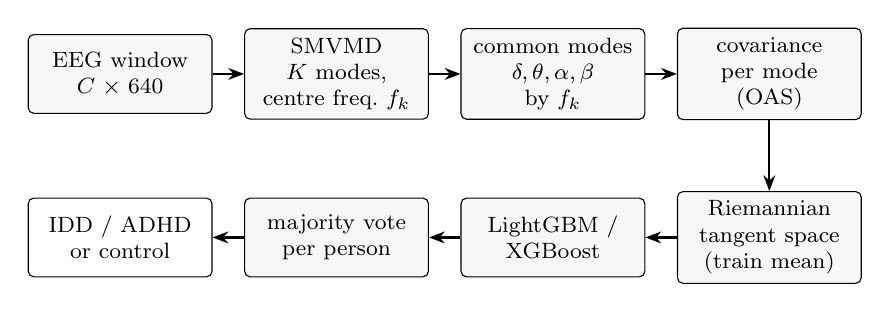
\begin{tikzpicture}[node distance=4mm and 4mm, font=\footnotesize,
  box/.style={draw, rounded corners=2pt, align=center, minimum height=10mm, text width=21mm,
              fill=gray!6},
  arr/.style={-{Stealth[length=2mm]}, thick}]
\node[box] (x) {EEG window\\$C\times 640$};
\node[box, right=of x] (s) {SMVMD\\$K$ modes,\\centre freq.\ $f_k$};
\node[box, right=of s] (c) {common modes\\$\delta,\theta,\alpha,\beta$\\by $f_k$};
\node[box, right=of c] (v) {covariance\\per mode\\(OAS)};
\node[box, below=9mm of v] (t) {Riemannian\\tangent space\\(train mean)};
\node[box, left=of t] (g) {LightGBM /\\XGBoost};
\node[box, left=of g] (m) {majority vote\\per person};
\node[box, left=of m, fill=white] (d) {IDD / ADHD\\or control};
\draw[arr] (x) -- (s); \draw[arr] (s) -- (c); \draw[arr] (c) -- (v); \draw[arr] (v) -- (t);
\draw[arr] (t) -- (g); \draw[arr] (g) -- (m); \draw[arr] (m) -- (d);
\end{tikzpicture}
\caption{The proposed pipeline. The upper row is computed independently for each window and uses
no labels; the lower row is learned from the training subjects of each fold.}
\label{fig:pipeline}
\end{figure}

\section{Successive multivariate variational mode decomposition}
\textbf{Variational mode decomposition.} VMD~\cite{dragomiretskiy2014} represents a signal $x(t)$
as a sum of $K$ modes $u_k(t)$, each compact around a centre frequency $\omega_k$, by solving
\begin{equation}
\min_{\{u_k\},\{\omega_k\}} \sum_{k=1}^{K}
\left\| \partial_t\!\left[\left(\delta(t)+\frac{j}{\pi t}\right) * u_k(t)\right] e^{-j\omega_k t}
\right\|_2^2
\quad\text{s.t.}\quad \sum_{k} u_k(t) = x(t).
\end{equation}
The term in brackets is the analytic signal of the mode; shifting it by $e^{-j\omega_k t}$ to
baseband and penalising the energy of its derivative measures the bandwidth of the mode. In the
Fourier domain the solution for a mode is a Wiener-type filter of the signal centred at
$\omega_k$, and the centre frequency is the power-weighted mean frequency of the mode.

\textbf{Multivariate extension.} For a $C$-channel signal, MVMD~\cite{rehman2019} looks for
multivariate modes $\mathbf{u}_k(t)\in\mathbb{R}^C$ whose channels share one centre frequency
$\omega_k$. This alignment is essential here: the $c$-th channel of mode $k$ describes the same
oscillation at every electrode, so the covariance between channels within one mode is meaningful.

\textbf{Successive extraction.} VMD and MVMD need $K$ in advance. SMVMD~\cite{liu2022} extracts
the modes one at a time from the residual: the first mode is extracted from the window, then the
next from what remains, and so on, until the residual energy falls below 1\% of the window
energy or 20 modes have been extracted. In the implementation used here (the same as for the
starting method), mode $k$ is obtained from the residual spectrum $\hat{r}_c(\nu)$ of each
channel $c$, with $\nu\in[0,\tfrac12]$ the normalised frequency in cycles per sample, by
iterating
\begin{equation}
\hat{u}_{k,c}(\nu) = \frac{\hat{r}_c(\nu)}{1 + 2\alpha(\nu-\nu_k)^2},
\qquad
\nu_k = \frac{\sum_c \sum_{\nu} \nu\, |\hat{u}_{k,c}(\nu)|^2}
             {\sum_c \sum_{\nu} |\hat{u}_{k,c}(\nu)|^2},
\label{eq:smvmd}
\end{equation}
for at most 500 iterations or until $\nu_k$ changes by less than $10^{-10}$, after which the mode
is subtracted from the residual. The common centre frequency $\nu_k$, shared by all channels, is
what makes the modes multivariate. The parameter $\alpha$ sets the bandwidth of the modes ($\alpha=2000$ for DS-1 and
$1000$ for DS-2, as for the starting method~\cite{chandela2025}), and the dual-ascent step is set
to zero, so the modes do not have to reconstruct the noisy signal exactly. Because the number of
modes adapts to the signal, it differs between windows: on average \R{CmDSoneRestMusicModesMean}
modes per DS-1 window (range \R{CmDSoneRestMusicModesMin}--\R{CmDSoneRestMusicModesMax}) and
\R{CmDStwoModesMean} per DS-2 window (range \R{CmDStwoModesMin}--\R{CmDStwoModesMax}).

\section{Common modes}
A classifier needs the same features for every window, but SMVMD gives each window its own
number of modes at its own frequencies (Fig.~\ref{fig:centrefreq}). The starting method solved
this by averaging the features of all modes with energy weights, which discards the frequency
information. The proposed pipeline instead assigns every mode to a fixed frequency band by its
centre frequency in hertz, $f_k=\nu_k f_s$ with $f_s=128$~Hz, and sums the modes within each
band:
\begin{equation}
\mathbf{U}_b = \sum_{k:\; f_k\in B_b} \mathbf{u}_k,\qquad
B_\delta=[0,4),\; B_\theta=[4,8),\; B_\alpha=[8,13),\; B_\beta=[13,30)\ \text{Hz}.
\label{eq:common}
\end{equation}
The four components $\mathbf{U}_\delta,\mathbf{U}_\theta,\mathbf{U}_\alpha,\mathbf{U}_\beta \in
\mathbb{R}^{C\times T}$ are the \emph{common modes} of the window. Unlike the outputs of fixed
band-pass filters, they are built from the window's own oscillatory components: a common mode
contains the modes that SMVMD found in that band, with the bandwidth and centre that fit the
window, and nothing where SMVMD found no oscillation. The band edges are the conventional EEG
bands, chosen before any result was seen. Modes at 30~Hz and above are not used: DS-1 was
band-limited to 1--30~Hz by its authors, and in DS-2 such modes carry on average only
\R{CmDStwoShareAbove}\% of the mode energy. A fifth component, the sum of all modes (the SMVMD
reconstruction), is used only in the ablation.

\begin{figure}[H]\centering
\genfig[0.95\textwidth]{centre_frequencies}
\caption{Centre frequencies of all SMVMD modes of all windows. Dashed lines: the edges of the
common modes (4, 8, 13 and 30~Hz).}
\label{fig:centrefreq}
\end{figure}

Table~\ref{tab:commonmodes} summarises the common modes. In DS-1 the energy is shared between the
$\delta$ and $\alpha$ modes, consistent with relaxed wakefulness during the rest and music
recordings. In DS-2 nearly all energy lies in the $\delta$ mode, and many windows contain no mode
in the $\alpha$ (\R{CmDStwoEmptyAlpha}\% of windows) or $\beta$ (\R{CmDStwoEmptyBeta}\%) band.

\begin{table}[H]
\caption{Common modes: modes per window (mean and range), and per band the mean share of mode
energy (\%) / the percentage of windows without any mode in that band.}
\label{tab:commonmodes}\centering
\gentable{tab_common_modes}
\end{table}

\section{Covariance estimation}
Each common mode is summarised by its spatial covariance matrix. With
$\mathbf{S}_b=\frac{1}{T}\mathbf{U}_b\mathbf{U}_b^{\top}$ the sample covariance (the modes have
zero mean), the oracle approximating shrinkage (OAS) estimator~\cite{chen2010}
\begin{equation}
\boldsymbol{\Sigma}_b = (1-\rho)\,\mathbf{S}_b + \rho\,\frac{\operatorname{tr}(\mathbf{S}_b)}{C}\,\mathbf{I}
\end{equation}
shrinks it towards a scaled identity, with the weight $\rho$ computed in closed form from
$\mathbf{S}_b$. Shrinkage keeps the matrix well conditioned, which matters for DS-1, whose
cleaned recordings are rank-deficient after the removal of independent components. When a window
has no mode in a band, $\mathbf{U}_b=\mathbf{0}$; to keep every matrix positive definite, a floor
$\epsilon\,\bar{p}\,\mathbf{I}$ is added to all matrices, where $\bar{p}$ is the mean channel power
of the whole window and $\epsilon=10^{-4}$. The covariance of a window depends only on that
window, so these matrices are computed once, before cross-validation.

The covariance matrix captures two kinds of information: the diagonal holds the power of each
channel in the band, and the off-diagonal entries hold the co-variation of pairs of channels,
that is, the spatial structure of the oscillation. Per-channel features such as band powers
contain only the first kind.

\section{Riemannian geometry of covariance matrices}
\textbf{The SPD manifold.} Covariance matrices are symmetric positive definite (SPD). They do not
form a vector space: the difference of two SPD matrices need not be SPD, and the Euclidean mean
of SPD matrices is inflated (the ``swelling effect''). The set of SPD matrices is a Riemannian
manifold, and the natural distance on it, the affine-invariant Riemannian distance,
\begin{equation}
\delta_R(\boldsymbol{\Sigma}_1,\boldsymbol{\Sigma}_2) =
\left\| \log\!\left(\boldsymbol{\Sigma}_1^{-1/2}\boldsymbol{\Sigma}_2\boldsymbol{\Sigma}_1^{-1/2}\right)\right\|_F
= \Big(\sum_{i=1}^{C} \log^2 \lambda_i\Big)^{1/2},
\end{equation}
where $\lambda_i$ are the eigenvalues of $\boldsymbol{\Sigma}_1^{-1}\boldsymbol{\Sigma}_2$, is
invariant to any invertible linear transformation of the channels:
$\delta_R(\mathbf{A}\boldsymbol{\Sigma}_1\mathbf{A}^\top, \mathbf{A}\boldsymbol{\Sigma}_2\mathbf{A}^\top)
=\delta_R(\boldsymbol{\Sigma}_1,\boldsymbol{\Sigma}_2)$~\cite{barachant2012, congedo2017}. Since
the scalp EEG is a linear mixture of cortical sources, this invariance makes the geometry well
suited to EEG.

\textbf{Riemannian mean.} The mean of a set of matrices $\{\boldsymbol{\Sigma}_i\}$ is the point
$\mathbf{M}$ that minimises $\sum_i \delta_R^2(\mathbf{M},\boldsymbol{\Sigma}_i)$. It has no closed
form and is computed by a fixed-point iteration that alternately maps the matrices to the tangent
space at the current estimate, averages them there and maps the average back to the manifold.

\textbf{Tangent-space mapping.} Near a reference point $\mathbf{M}$, the manifold is approximated
by its tangent space, which is a vector space. Each matrix is mapped to a vector by
\begin{equation}
\mathbf{s} = \operatorname{upper}\!\left(\log\!\left(\mathbf{M}^{-1/2}\boldsymbol{\Sigma}\,\mathbf{M}^{-1/2}\right)\right),
\label{eq:ts}
\end{equation}
where $\operatorname{upper}(\cdot)$ keeps the $C(C+1)/2$ entries of the upper triangle and
multiplies the off-diagonal entries by $\sqrt{2}$, so that the Euclidean norm of $\mathbf{s}$
equals the Riemannian distance between $\boldsymbol{\Sigma}$ and $\mathbf{M}$. The reference
$\mathbf{M}$ is the Riemannian mean of the \emph{training} windows of the fold, computed
separately for each common mode. The four tangent vectors are concatenated into one feature
vector of length $4\cdot C(C+1)/2$: \R{RtFeatures} features for DS-2 ($C=19$) and 420 for DS-1
($C=14$).

\section{Gradient-boosted decision trees}
The tangent vectors are classified with gradient-boosted decision trees~\cite{chen2016, ke2017}.
The model is an additive ensemble $F(\mathbf{s})=\sum_{m=1}^{M} \eta\, f_m(\mathbf{s})$ of $M$
regression trees, and the probability of the disorder is $\sigma(F(\mathbf{s}))$. Trees are
added one at a time; tree $f_m$ is fitted to the gradient (and, in XGBoost and LightGBM, the
curvature) of the logistic loss of the current ensemble, so that each tree corrects the errors of
the previous ones. Gradient boosting was chosen over the logistic regression and SVM used in the
preliminary study for three reasons: trees model interactions between features, here between
channel pairs and between modes, without a kernel choice; they are insensitive to the scale and
to outlying values of individual features, such as the floored covariances of empty modes; and
they train in seconds and give a feature importance that can be traced back to modes and
electrodes.

\textbf{LightGBM}~\cite{ke2017} grows trees leaf-wise on histogram-binned features, and
\textbf{XGBoost}~\cite{chen2016} grows them level-wise with a regularised objective. Both are
used with the same budget, fixed in advance: $M=300$ trees, learning rate $\eta=0.05$, a random
80\% of the windows and 50\% of the features per tree, and class weights inversely proportional
to the class frequencies of the training windows. The tree depth is chosen from $\{2, 4\}$ by the
inner cross-validation (for LightGBM the number of leaves is $2^{\text{depth}}-1$). The features
are standardised with the mean and standard deviation of the training windows.

\section{Choice of the common modes}
Which common modes should be used may differ between disorders, so the mode set is part of the
model and is chosen by the inner cross-validation, together with the tree depth. The candidates
are each single mode and all four together, giving $5\times 2=10$ grid points. In each outer
fold, an inner stratified grouped 4-fold cross-validation over the training subjects evaluates
every grid point, the point with the highest pooled balanced accuracy is selected, and the model
is refitted on the whole outer training set. The test subjects of the outer fold play no part in
this choice.

\section{Decision per person}
The pipeline classifies every window. A person is assigned the class of the majority of their
windows, with ties broken by the mean predicted probability.

\section{What is fitted where}
\begin{table}[H]
\caption{Where each part of the pipeline is computed. ``Per window'' parts use one window and no
labels; ``training subjects'' parts are refitted in every outer fold.}
\label{tab:fitted}\centering\small
\begin{tabular}{lll}
\hline
Stage & Computed from & Leakage possible? \\
\hline
SMVMD, common modes & each window alone & no \\
OAS covariance and floor & each window alone & no \\
Riemannian mean (tangent-space reference) & training subjects of the fold & no \\
Standardisation & training subjects of the fold & no \\
Mode set and tree depth & inner CV on training subjects & no \\
Gradient-boosted trees & training subjects of the fold & no \\
Majority vote & the test person's own predictions & no \\
\hline
\end{tabular}
\end{table}

\section{Computational cost}
\label{sec:cost}
On the laptop CPU used for this work (one core per stage), processing one 5-second window takes
about \R{RtSmvmd}~ms for SMVMD, \R{RtCov}~ms for the four covariance matrices and \R{RtPred}~ms for
the tangent-space mapping and LightGBM prediction, \R{RtTotal}~ms in total, about
\R{RtRealtime} times faster than real time. Training one model on \R{RtTrainWin} DS-2 windows
takes about \R{RtTrain}~s; the trained model has \R{RtTrees} trees with \R{RtLeaves} leaves in
total and occupies about \R{RtModelKB}~kB. No GPU is needed at any stage. SMVMD dominates the
cost; in the experiments it was run in parallel over windows.

\section{Implementation}
The pipeline is implemented in Python with NumPy and SciPy (SMVMD, filters), pyRiemann (OAS
covariance, Riemannian mean, tangent space), scikit-learn~\cite{pedregosa2011} (standardisation,
logistic regression, SVM, cross-validation), XGBoost and LightGBM. The experiments are in
\texttt{experiments/stage2c\_smvmd\_riemann.py} and \texttt{experiments/stage2d\_main\_pipeline.py}
(Appendix~B).

\chapter{Results and Discussion}
\thispagestyle{empty}

All results in this chapter are obtained on people not seen during training, with the protocol of
Chapter~4: leave-one-subject-out for DS-1 (14 folds) and stratified grouped 10-fold
cross-validation for DS-2, with nested tuning on the training subjects. Balanced accuracy is per
window; ``subjects'' or ``children'' counts the people
classified correctly by majority vote.

\section{Main results}
Table~\ref{tab:main} gives the results of the proposed pipeline (SMVMD common modes, Riemannian
tangent space and LightGBM, with the mode set chosen by the inner cross-validation).

\begin{table}[H]
\caption{The proposed pipeline on unseen people. Window-level balanced accuracy with 95\% CI over
subjects, AUC, sensitivity and specificity (\%), and people classified correctly by majority
vote.}
\label{tab:main}\centering
\gentable{tab_main}\\[2pt]
{\footnotesize \dstwonote}
\end{table}

\textbf{ADHD (DS-2).} The pipeline reaches \R{MainDStwoBal}\% balanced accuracy (95\% CI
\R{MainDStwoBalCI}\%) and an AUC of \R{MainDStwoAUC} on the windows of unseen children, and
classifies \R{MainDStwoSubj} children correctly (\R{MainDStwoSubjAcc}\%). Sensitivity (\R{MainDStwoSens}\%) is
higher than specificity (\R{MainDStwoSpec}\%): control windows are misclassified more often than
ADHD windows. In every outer fold the inner cross-validation chose all four common modes
together (\R{MainDStwoChosen}).

\textbf{IDD (DS-1).} All 14 participants are classified correctly in all three settings, with
balanced window accuracies of \R{MainDSoneRestBal}\% (rest), \R{MainDSoneMusicBal}\% (music) and
\R{MainDSoneRestMusicBal}\% (rest and music). Here the inner
cross-validation mostly chose the $\alpha$ mode alone (Table~\ref{tab:chosen}): the two
disorders are detected from different frequency ranges by the same pipeline. Because the two DS-1
groups are also separated by a single property of the rest recordings, their relative beta power
(AUC \R{DSoneRestRelBetaAUC}, Section~\ref{sec:datachecks}), and have only seven adults each,
the DS-1 result shows that the pipeline transfers to a second disorder, not that it has found an
EEG marker of IDD.

\begin{table}[H]
\caption{Common-mode set chosen by the inner cross-validation in the outer folds.}
\label{tab:chosen}\centering
\gentable{tab_chosen}
\end{table}

\section{Choice of classifier}
Table~\ref{tab:classifiers} and Fig.~\ref{fig:classifiers} compare four classifiers on the same
tangent-space features of DS-2, for the SMVMD common modes and, for reference, for the broadband
covariance of the undecomposed window (the representation of Step~7).

\begin{table}[H]
\caption{DS-2: classifier comparison on tangent-space features. Balanced window accuracy (\%),
AUC, and children correct.}
\label{tab:classifiers}\centering
\gentable{tab_classifiers}\\[2pt]
{\footnotesize \dstwonote}
\end{table}

\begin{figure}[H]\centering
\genfig[0.9\textwidth]{classifier_comparison}
\caption{DS-2: balanced accuracy of the four classifiers on three tangent-space representations.
Error bars: 95\% CI over children; dashed line: chance.}
\label{fig:classifiers}
\end{figure}

Gradient boosting improves on the linear and kernel classifiers for the SMVMD common modes: with
the mode set chosen in the training folds, logistic regression reaches \R{AblSelectLrBal}\%, the
SVM \R{AblSelectSvmBal}\%, XGBoost \R{AblSelectXgbBal}\% and LightGBM \R{AblSelectLgbmBal}\%, and
LightGBM classifies the most children correctly (\R{AblSelectLgbmSubj}). On the broadband
covariance, LightGBM also gives the highest score (\R{AblRawLgbmBal}\%, \R{AblRawLgbmSubj}
children), while XGBoost is there slightly below the SVM. All these differences are small, a few
points at most; the classifiers should be regarded as close to equivalent, with LightGBM the
highest on both representations.

\section{Contribution of the modes and of the decomposition}
Table~\ref{tab:modes} and Fig.~\ref{fig:modes} show, for DS-2, the result of each common mode on
its own, of all four, and of the sum of all modes, and compare the SMVMD common modes with
zero-phase Butterworth band-pass filters with the same band edges, under an otherwise identical
pipeline (LR and SVM, which were run for every variant).

\begin{table}[H]
\caption{DS-2: balanced window accuracy (\%) of single and combined components, SMVMD common
modes against Butterworth bands with the same edges.}
\label{tab:modes}\centering
\gentable{tab_modes}\\[2pt]
{\footnotesize \dstwonote}
\end{table}

\begin{figure}[H]\centering
\genfig[0.85\textwidth]{mode_comparison}
\caption{DS-2, SVM: balanced accuracy of each SMVMD common mode and Butterworth band, and of all
four together. Grey line: undecomposed broadband covariance (Step~7). Error bars: 95\% CI.}
\label{fig:modes}
\end{figure}

Three observations follow. First, the slow modes carry most of the information about ADHD: the
$\delta$ mode alone reaches \R{ModeDeltaSVMBal}\% with the SVM, the $\theta$ mode
\R{ModeThetaSVMBal}\%, while the $\alpha$ (\R{ModeAlphaSVMBal}\%) and $\beta$
(\R{ModeBetaSVMBal}\%) modes are weaker, in line with the many DS-2 windows in which SMVMD finds
no mode in these bands (Table~\ref{tab:commonmodes}). Second, the SMVMD reconstruction gives the
same result as the undecomposed window (\R{ModeReconSVMBal}\%), because the reconstruction
contains almost all of the signal and therefore has nearly the same covariance. Third, fixed
Butterworth bands perform at least as well as the SMVMD common modes overall: the SMVMD
$\delta$ mode is better than the Butterworth $\delta$ band, but in the $\alpha$ and $\beta$
bands, where SMVMD often finds no mode, the filters are better, and with all four components
together the filter bank is slightly ahead. \emph{The adaptive decomposition therefore makes the frequency-specific covariance
representation possible, but it does not by itself add accuracy}; this agrees with the
preliminary finding that features of the raw signal do as well as features of the SMVMD modes
(Chapter~5). Its value in the pipeline lies in a data-driven, interpretable split of the signal
into the oscillations actually present in each window, at an accuracy only one to two points
below the best fixed representations.

\section{Effect of window-level splitting on the proposed pipeline}
To show how the pipeline would be reported under the window-level protocol common in the
literature, the same configuration (all four modes, LightGBM of depth 4) was evaluated with
10-fold cross-validation over windows (Table~\ref{tab:gapmain}). On DS-2 the window-level
protocol reports \R{GapDStwoLeaky}\% against \R{GapDStwoSubj}\% on unseen children, an inflation
of \R{GapDStwoPoints} percentage points. The figures in the 95--100\% range in the literature
(Table~\ref{tab:lit}) are therefore not comparable with subject-wise results, and the proposed
pipeline would itself appear above 90\% if it were evaluated in the same way. On DS-1 the
inflation is small (\R{GapDSoneRestPoints} points) only because the subject-wise result is
already close to 100\%.

\begin{table}[H]
\caption{The proposed pipeline (fixed configuration) under window-wise and subject-wise
cross-validation: balanced window accuracy (\%).}
\label{tab:gapmain}\centering
\gentable{tab_gap_main}\\[2pt]
{\footnotesize \dstwonote}
\end{table}

\section{What the pipeline relies on}
Fig.~\ref{fig:importance} shows the LightGBM importance (total gain, averaged over the 10 outer
DS-2 models) summed per common mode and per electrode, and Table~\ref{tab:topfeat} the ten most
important tangent-space features.

\begin{figure}[H]\centering
\genfig[0.95\textwidth]{importance_main}
\caption{DS-2: share of LightGBM gain per common mode (left) and per electrode (right; the gain
of a channel pair is divided equally between its two electrodes).}
\label{fig:importance}
\end{figure}

\begin{table}[H]
\caption{DS-2: the ten most important tangent-space features of the proposed pipeline. A
``variance'' feature is a diagonal element (power of one channel in the mode), a ``covariance''
feature an off-diagonal element (co-variation of two channels).}
\label{tab:topfeat}\centering
\gentable{tab_top_features}
\end{table}

For ADHD the $\delta$ mode receives \R{ImpDStwoDelta}\% of the importance and the $\theta$ mode
\R{ImpDStwoTheta}\%, against \R{ImpDStwoAlpha}\% and \R{ImpDStwoBeta}\% for the $\alpha$ and $\beta$
modes, in agreement with the single-mode results. Off-diagonal (covariance) features account for
\R{ImpDStwoCovShare}\% of the total importance and diagonal (power) features for
\R{ImpDStwoVarShare}\%. Since the off-diagonal elements are 90\% of the features (171 of 190 per
mode), a single power feature is on average more important than a single channel pair; but most
of the information the classifier uses comes from the co-variation of channels, which per-channel
features cannot capture, consistent with the advantage of connectivity and Riemannian features in
the preliminary study. The most important electrodes are \R{ImpDStwoTopChannels}. Slow activity at frontal electrodes such as Fp2
is also where residual eye-movement artefacts appear, and stimulant medication, which only the
ADHD group received, changes the EEG in the theta band among others~\cite{clarke2002}; the
importance pattern is therefore compatible with both a neural and a non-neural explanation and
should not be read as a biomarker.

\section{Comparison with published results}
Table~\ref{tab:litcomp} places the proposed pipeline beside the published subject-wise results
on the same ADHD dataset (Chapter~2).

\begin{table}[H]
\caption{ADHD dataset: subject-wise results. Published values as reported (accuracy); this work:
balanced accuracy and plain window accuracy.}
\label{tab:litcomp}\centering\small
\begin{adjustbox}{max width=\textwidth}
\begin{tabular}{p{5.6cm}p{3.6cm}p{2.0cm}r}
\hline
Method & Evaluation & Model type & Accuracy (\%) \\
\hline
SVM on spectral features~\cite{geethapriya2026} & subject-wise 10-fold & shallow & 65.6 \\
LSTM~\cite{geethapriya2026} & subject-wise 10-fold & deep (recurrent) & 61.6 \\
CNN--BiLSTM~\cite{geethapriya2026} & subject-wise 10-fold & deep & 65.7 \\
CNN~\cite{geethapriya2026} & subject-wise 10-fold & deep & 72.7 \\
\hline
Starting method, this work (Step~1) & subject-wise 10-fold & shallow & \R{StepADStwoBal} (bal.) \\
\textbf{Proposed pipeline (this work)} & subject-wise 10-fold & \textbf{shallow, CPU} & \textbf{\R{MainDStwoBal}} (bal.) \\
 & & & \R{MainDStwoWinAccPlain} (acc.) \\
\hline
\end{tabular}
\end{adjustbox}\\[2pt]
{\footnotesize \dstwonote}
\end{table}

The proposed pipeline scores higher than the recurrent and hybrid deep networks and the spectral
SVM evaluated subject-wise on the same data, and it is comparable with the best published
subject-wise result, a convolutional network trained end to end, from which it differs by about
one point. The comparison is approximate, since the window length
(5~s with overlap against 4~s without), the folds and the measure (balanced against plain
accuracy) differ. The advantages of the proposed pipeline are of a different kind: it needs no
GPU and no deep network, processes a window in about \R{RtTotal}~ms on one CPU core, trains in
about \R{RtTrain}~s, applies unchanged to a second disorder, and its decisions can be traced to
frequency modes and electrode pairs.

\section{Discussion}
\textbf{Medication and other confounds (DS-2).} The children with ADHD were taking
methylphenidate and the controls were not. Stimulants change the EEG, mainly in the theta and
beta bands~\cite{clarke2002}, and the $\theta$ mode is the second most important mode of the
pipeline. In addition, recordings of children with ADHD are longer (\R{DStwoLenAdhd} against
\R{DStwoLenCtrl} windows on average) because the task lasted until the child answered, and
recording length alone predicts the group with an AUC of \R{DStwoLenAUC}; anything in the signal
that reflects how long or how hard the task was for a child is therefore also a cue. The result
is the detection of medicated ADHD against unmedicated controls, and could partly reflect the
medication or task performance.

\textbf{Uncertainty and selection.} The confidence interval of the main DS-2 result,
\R{MainDStwoBalCI}\%, is about ten points wide, so differences of one or two points between
pipelines are not meaningful. The pipeline's configuration was fixed before its final result was
seen, and its mode set was chosen in the training folds; the per-mode and per-classifier rows of
the ablations are analyses, and the best of them is slightly optimistic. The undecomposed
Riemannian pipeline with LightGBM (\R{AblRawLgbmBal}\%) is numerically the highest single result
of the study, but it is not distinguishable from the proposed pipeline.

\textbf{Diagnostic value.} About three in four unseen children are classified correctly. This is
a substantial and honest improvement over the starting method and comparable with the best
published subject-wise result, but it is far from the accuracy needed for diagnosis, and the
pipeline is a research result, not a clinical tool.

\chapter{Conclusions, Limitations and Future Work}
\thispagestyle{empty}

\section{Conclusions}
This project developed an EEG pipeline for the detection of two neurodevelopmental disorders,
IDD and ADHD, with one common processing chain, and evaluated it strictly on people the model had
never seen. The main conclusions are as follows.

\begin{enumerate}
\item \textbf{The proposed pipeline detects both disorders on unseen people.} SMVMD common
      modes, their channel covariances in the Riemannian tangent space and LightGBM reach
      \R{MainDStwoBal}\% balanced accuracy and
      \R{MainDStwoSubj} children correct on ADHD, and classify all 14 participants correctly
      in all three IDD settings.
\item \textbf{It improves substantially on the best-reported method and matches the best
      published subject-wise result.} The starting method reaches \R{StepADStwoBal}\% on unseen
      ADHD children. The proposed pipeline is comparable with the best published subject-wise
      result on the same data, a deep convolutional network, while needing no GPU, about
      \R{RtTotal}~ms per window on one CPU core and about \R{RtTrain}~s of training.
\item \textbf{The channel covariance carries the information.} Representations that describe
      how channels co-vary (connectivity, Riemannian tangent space) outperform per-channel
      features, and most of the pipeline's importance lies in channel pairs.
\item \textbf{Gradient-boosted trees suit the tangent-space features.} LightGBM gives the highest
      score for the proposed configuration and for the undecomposed covariance, and both
      boosting libraries are ahead of logistic regression on every representation, although the
      differences between classifiers are small.
\item \textbf{The two disorders use different modes.} The inner cross-validation chose all four
      modes, dominated by $\delta$ and $\theta$, for ADHD, and mainly the $\alpha$ mode for IDD.
\item \textbf{The adaptive decomposition does not add accuracy by itself.} Fixed band-pass
      filters and the undecomposed signal perform as well or one to two points better; SMVMD's
      role is to provide an interpretable, data-driven split of
      each window into the oscillations it contains.
\item \textbf{Evaluation on new people is essential.} The proposed pipeline itself would be
      reported at \R{GapDStwoLeaky}\% on ADHD under window-level cross-validation, against
      \R{GapDStwoSubj}\% on unseen children; accuracies of 95--100\% in the literature are
      not comparable with subject-wise results.
\end{enumerate}

\section{Limitations}
\begin{itemize}
\item \textbf{Medication confound.} The ADHD children were medicated and the controls were not,
      so the ADHD results cannot be attributed to ADHD alone.
\item \textbf{Small IDD sample.} DS-1 has 14 adult participants; one participant changes the
      subject accuracy by about 7 points, so even 14/14 is a weak estimate, and the groups may
      differ in recording conditions, artefacts and age as well as in the disorder.
\item \textbf{One dataset per disorder.} Each disorder is represented by a single dataset with its
      own device, task and population, so a single model distinguishing the two disorders could
      not be evaluated meaningfully.
\item \textbf{No external validation.} No independent cohort was available, and nothing here
      supports clinical use.
\item \textbf{Fixed band edges.} The common modes use the conventional EEG bands; edges adapted to
      the data were not explored.
\end{itemize}

\section{Future work}
\begin{itemize}
\item \textbf{Better data}: both groups recorded under the same protocol and device, matched in
      age, with medication status recorded and ideally a washout period; for IDD, a cohort of
      children.
\item \textbf{External validation} of the frozen pipeline on an independent ADHD cohort.
\item \textbf{Data-driven common modes}: band edges learned from the distribution of SMVMD
      centre frequencies in the training data, or a weighting of the modes instead of a hard
      assignment.
\item \textbf{Subject-invariant representations}: Riemannian re-centring or other alignment of
      each person's covariances, which address the differences between individuals that limit
      all methods.
\item \textbf{Faster decomposition}: SMVMD accounts for almost all of the computation; a
      filter bank derived from the training-set mode frequencies would make the pipeline
      suitable for real-time use on a headset.
\item \textbf{More disorders}: extending the pipeline to autism spectrum disorder under the same
      protocol.
\end{itemize}


\newpage
\addcontentsline{toc}{chapter}{References}
\begin{thebibliography}{99}

\bibitem{apa2013} American Psychiatric Association, \emph{Diagnostic and Statistical Manual of
Mental Disorders}, 5th ed. Arlington, VA, USA: American Psychiatric Publishing, 2013.

\bibitem{polanczyk2007} G. Polanczyk, M. S. de Lima, B. L. Horta, J. Biederman, and L. A.
Rohde, ``The worldwide prevalence of ADHD: A systematic review and metaregression analysis,''
\emph{Am. J. Psychiatry}, vol.~164, no.~6, pp.~942--948, 2007.

\bibitem{maulik2011} P. K. Maulik, M. N. Mascarenhas, C. D. Mathers, T. Dua, and S. Saxena,
``Prevalence of intellectual disability: A meta-analysis of population-based studies,''
\emph{Res. Dev. Disabil.}, vol.~32, no.~2, pp.~419--436, 2011.

\bibitem{chandela2025} U. Chandela, K. N. Faisal, and R. R. Sharma, ``Electroencephalogram-based
unified approach for multiple neurodevelopmental disorders detection in children using
successive multivariate variational mode decomposition,'' \emph{IEEE Trans. Cogn. Develop.
Syst.}, vol.~17, no.~6, pp.~1350--1359, Dec. 2025.

\bibitem{sareen2020data} E. Sareen, L. Singh, B. Varkey, K. Achary, and A. Gupta, ``EEG
dataset of individuals with intellectual and developmental disorder and healthy controls
under rest and music stimuli,'' \emph{Data Brief}, vol.~30, 2020, Art. no.~105488.

\bibitem{motie2020} A. Motie Nasrabadi, A. Allahverdy, M. Samavati, and M. R. Mohammadi,
``EEG data for ADHD/control children,'' IEEE DataPort, 2020, doi: 10.21227/rzfh-zn36.

\bibitem{snyder2006} S. M. Snyder and J. R. Hall, ``A meta-analysis of quantitative EEG power
associated with attention-deficit hyperactivity disorder,'' \emph{J. Clin. Neurophysiol.},
vol.~23, no.~5, pp.~440--455, 2006.

\bibitem{arns2013} M. Arns, C. K. Conners, and H. C. Kraemer, ``A decade of EEG theta/beta
ratio research in ADHD: A meta-analysis,'' \emph{J. Atten. Disord.}, vol.~17, no.~5,
pp.~374--383, 2013.

\bibitem{clarke2002} A. R. Clarke, R. J. Barry, D. Bond, R. McCarthy, and M. Selikowitz,
``Effects of stimulant medications on the EEG of children with attention-deficit/hyperactivity
disorder,'' \emph{Psychopharmacology}, vol.~164, no.~3, pp.~277--284, 2002.

\bibitem{huang1998} N. E. Huang \emph{et al.}, ``The empirical mode decomposition and the
Hilbert spectrum for nonlinear and non-stationary time series analysis,'' \emph{Proc. R. Soc.
Lond. A}, vol.~454, pp.~903--995, 1998.

\bibitem{dragomiretskiy2014} K. Dragomiretskiy and D. Zosso, ``Variational mode
decomposition,'' \emph{IEEE Trans. Signal Process.}, vol.~62, no.~3, pp.~531--544, Feb. 2014.

\bibitem{rehman2019} N. Ur Rehman and H. Aftab, ``Multivariate variational mode
decomposition,'' \emph{IEEE Trans. Signal Process.}, vol.~67, no.~23, pp.~6039--6052, Dec. 2019.

\bibitem{liu2022} S. Liu and K. Yu, ``Successive multivariate variational mode
decomposition,'' \emph{Multidimensional Syst. Signal Process.}, vol.~33, no.~3,
pp.~917--943, 2022.

\bibitem{peng2005} H. Peng, F. Long, and C. Ding, ``Feature selection based on mutual
information: Criteria of max-dependency, max-relevance, and min-redundancy,'' \emph{IEEE
Trans. Pattern Anal. Mach. Intell.}, vol.~27, no.~8, pp.~1226--1238, Aug. 2005.

\bibitem{cover1967} T. Cover and P. Hart, ``Nearest neighbor pattern classification,''
\emph{IEEE Trans. Inf. Theory}, vol.~13, no.~1, pp.~21--27, 1967.

\bibitem{welch1967} P. Welch, ``The use of fast Fourier transform for the estimation of power
spectra: A method based on time averaging over short, modified periodograms,'' \emph{IEEE
Trans. Audio Electroacoust.}, vol.~15, no.~2, pp.~70--73, 1967.

\bibitem{hjorth1970} B. Hjorth, ``EEG analysis based on time domain properties,''
\emph{Electroencephalogr. Clin. Neurophysiol.}, vol.~29, no.~3, pp.~306--310, 1970.

\bibitem{richman2000} J. S. Richman and J. R. Moorman, ``Physiological time-series analysis
using approximate entropy and sample entropy,'' \emph{Am. J. Physiol. Heart Circ. Physiol.},
vol.~278, no.~6, pp.~H2039--H2049, 2000.

\bibitem{bandt2002} C. Bandt and B. Pompe, ``Permutation entropy: A natural complexity measure
for time series,'' \emph{Phys. Rev. Lett.}, vol.~88, no.~17, Art. no.~174102, 2002.

\bibitem{donoghue2020} T. Donoghue \emph{et al.}, ``Parameterizing neural power spectra into
periodic and aperiodic components,'' \emph{Nat. Neurosci.}, vol.~23, pp.~1655--1665, 2020.

\bibitem{vinck2011} M. Vinck, R. Oostenveld, M. van Wingerden, F. Battaglia, and C. M. A.
Pennartz, ``An improved index of phase-synchronization for electrophysiological data in the
presence of volume-conduction, noise and sample-size bias,'' \emph{NeuroImage}, vol.~55, no.~4,
pp.~1548--1565, 2011.

\bibitem{chen2010} Y. Chen, A. Wiesel, Y. C. Eldar, and A. O. Hero, ``Shrinkage algorithms for
MMSE covariance estimation,'' \emph{IEEE Trans. Signal Process.}, vol.~58, no.~10,
pp.~5016--5029, 2010.

\bibitem{barachant2012} A. Barachant, S. Bonnet, M. Congedo, and C. Jutten, ``Multiclass
brain--computer interface classification by Riemannian geometry,'' \emph{IEEE Trans. Biomed.
Eng.}, vol.~59, no.~4, pp.~920--928, 2012.

\bibitem{congedo2017} M. Congedo, A. Barachant, and R. Bhatia, ``Riemannian geometry for
EEG-based brain--computer interfaces; a primer and a review,'' \emph{Brain-Comput.
Interfaces}, vol.~4, no.~3, pp.~155--174, 2017.

\bibitem{lawhern2018} V. J. Lawhern \emph{et al.}, ``EEGNet: A compact convolutional neural
network for EEG-based brain--computer interfaces,'' \emph{J. Neural Eng.}, vol.~15, no.~5,
Art. no.~056013, 2018.

\bibitem{schirrmeister2017} R. T. Schirrmeister \emph{et al.}, ``Deep learning with
convolutional neural networks for EEG decoding and visualization,'' \emph{Hum. Brain Mapp.},
vol.~38, no.~11, pp.~5391--5420, 2017.

\bibitem{roy2019} Y. Roy, H. Banville, I. Albuquerque, A. Gramfort, T. H. Falk, and J.
Faubert, ``Deep learning-based electroencephalography analysis: A systematic review,''
\emph{J. Neural Eng.}, vol.~16, no.~5, Art. no.~051001, 2019.

\bibitem{dempster2021} A. Dempster, D. F. Schmidt, and G. I. Webb, ``MiniRocket: A very fast
(almost) deterministic transform for time series classification,'' in \emph{Proc. ACM SIGKDD},
2021, pp.~248--257.

\bibitem{cortes1995} C. Cortes and V. Vapnik, ``Support-vector networks,'' \emph{Mach.
Learn.}, vol.~20, no.~3, pp.~273--297, 1995.

\bibitem{breiman2001} L. Breiman, ``Random forests,'' \emph{Mach. Learn.}, vol.~45, no.~1,
pp.~5--32, 2001.

\bibitem{chen2016} T. Chen and C. Guestrin, ``XGBoost: A scalable tree boosting system,'' in
\emph{Proc. ACM SIGKDD}, 2016, pp.~785--794.

\bibitem{ke2017} G. Ke, Q. Meng, T. Finley, T. Wang, W. Chen, W. Ma, Q. Ye, and T.-Y. Liu,
``LightGBM: A highly efficient gradient boosting decision tree,'' in \emph{Adv. Neural Inf.
Process. Syst.}, 2017, pp.~3146--3154.

\bibitem{geethapriya2026} M. Geethapriya and K. Pattabiraman, ``Subject-independent
classification of ADHD from pediatric EEG: A leakage-aware deep learning framework with
interpretable neurophysiological mapping,'' \emph{Front. Neurosci.}, vol.~20, 2026, Art.
no.~1925266, doi: 10.3389/fnins.2026.1925266.

\bibitem{maheshwari2025} S. Maheshwari, K. N. V. P. S. Rajesh, V. Kanhangad, U. R. Acharya, and
T. S. Kumar, ``Entropy difference-based EEG channel selection technique for automated detection
of ADHD,'' \emph{PLoS ONE}, vol.~20, no.~4, Art. no.~e0319487, 2025.

\bibitem{bansal2025} J. Bansal, G. Gangwar, M. Aljaidi, A. Alkoradees, and G. Singh,
``EEG-based ADHD classification using autoencoder feature extraction and ResNet with double
augmented attention mechanism,'' \emph{Brain Sci.}, vol.~15, no.~1, Art. no.~95, 2025.

\bibitem{mao2025} Y. Mao, X. Qi, L. He, S. Wang, Z. Wang, and F. Wang, ``Advanced machine
learning techniques reveal multidimensional EEG abnormalities in children with ADHD: A framework
for automatic diagnosis,'' \emph{Front. Psychiatry}, vol.~16, Art. no.~1475936, 2025.

\bibitem{saeb2017} S. Saeb, L. Lonini, A. Jayaraman, D. C. Mohr, and K. P. Kording, ``The need
to approximate the use-case in clinical machine learning,'' \emph{GigaScience}, vol.~6,
no.~5, 2017.

\bibitem{brookshire2024} G. Brookshire \emph{et al.}, ``Data leakage in deep learning studies of
translational EEG,'' \emph{Front. Neurosci.}, vol.~18, Art. no.~1373515, 2024.

\bibitem{varoquaux2018} G. Varoquaux, ``Cross-validation failure: Small sample sizes lead to
large error bars,'' \emph{NeuroImage}, vol.~180, pp.~68--77, 2018.

\bibitem{donoho1995} D. L. Donoho and I. M. Johnstone, ``Adapting to unknown smoothness via
wavelet shrinkage,'' \emph{J. Amer. Statist. Assoc.}, vol.~90, no.~432, pp.~1200--1224, 1995.

\bibitem{efron1993} B. Efron and R. J. Tibshirani, \emph{An Introduction to the Bootstrap}.
New York, NY, USA: Chapman \& Hall, 1993.

\bibitem{clopper1934} C. J. Clopper and E. S. Pearson, ``The use of confidence or fiducial
limits illustrated in the case of the binomial,'' \emph{Biometrika}, vol.~26, no.~4,
pp.~404--413, 1934.

\bibitem{pedregosa2011} F. Pedregosa \emph{et al.}, ``Scikit-learn: Machine learning in
Python,'' \emph{J. Mach. Learn. Res.}, vol.~12, pp.~2825--2830, 2011.

\end{thebibliography}


\appendix
\chapter{Implementation Details of the Starting Method}
\thispagestyle{empty}
The published description of the SMVMD method~\cite{chandela2025} leaves some details open. The
choices made in this project are listed here; the SMVMD settings are shared by the proposed
pipeline. The full list, with reasons, is in \texttt{docs/reproducibility\_notes.md}.

\begin{table}[H]
\caption{Implementation choices where the published description is incomplete.}
\label{tab:choices}\centering\small
\begin{tabular}{p{4.2cm}p{9.6cm}}
\hline
Item & Choice in this project \\
\hline
DS-1 preprocessing & The cleaned recordings distributed with the dataset are used; the
original EEGLAB processing (CleanLine, ICA, ADJUST) is MATLAB-only and was not re-run. \\
DS-2 filters & Fourth-order Butterworth band-pass, zero-phase. \\
DS-2 wavelet processing & Two Coiflet-3 level-6 steps (removal of the slowest component, then
SURE shrinkage). \\
SMVMD stopping rule & Stop when the residual energy is below 1\% of the window energy, with at
most 20 modes; \R{DSoneModesCapPct}\% of DS-1 windows reach the limit. \\
SMVMD initialisation & Centre frequencies initialised uniformly; at most 500 iterations per
mode. \\
Features of the starting method & Nine statistical features per mode and channel, integrated
over modes with energy weights; mutual information for mRMR estimated with nearest-neighbour
estimators. \\
KNN settings & Taken from the reported optimised settings; the Bayesian optimisation that
produced them was not re-run. A tuned variant is Step~2. \\
\hline
\end{tabular}
\end{table}

\chapter{Reproducing the Results}
\thispagestyle{empty}
All experiments are run from the root of the project repository with Python~3.13. Results are
cached, so a repeated command skips completed work.

The commands below produce every result in this report, in this order. Each line starting with
\texttt{\#} describes the command that follows it; a trailing \texttt{\textbackslash} means that
the command continues on the next line.

\begin{footnotesize}
\begin{verbatim}
# dependencies
pip install -r requirements.txt lightgbm

# SMVMD features of the starting method (Step 1)
python -m experiments.ds1_rest
python -m experiments.ds1_music
python -m experiments.ds1_rest_music
python -m experiments.ds2_adhd

# preliminary study (Chapter 5) and data properties (Chapter 3)
python -m experiments.stage1_eval
python -m experiments.stage2_baselines
python -m experiments.stage2b_sweep
python -m experiments.stage3_ablation
python -m experiments.data_checks

# SMVMD, common modes and covariance matrices of every window (cached)
python experiments/stage2c_smvmd_riemann.py --part covs
python experiments/stage2c_smvmd_riemann.py --part summary

# LR and SVM variants, single modes and Butterworth control
python experiments/stage2c_smvmd_riemann.py --part eval --clf lr svm

# proposed pipeline (LightGBM, XGBoost) and undecomposed reference
python experiments/stage2c_smvmd_riemann.py --part eval \
       --clf xgb lgbm --variants all select raw

# window-wise comparison, feature importance and run time
python experiments/stage2d_main_pipeline.py --part gap
python experiments/stage2d_main_pipeline.py --part importance
python experiments/stage2d_main_pipeline.py --part runtime

# automated leakage and metric tests
python -m pytest tests

# all numbers, tables and figures of this report
python report/build_final.py
python report/build_report2.py
\end{verbatim}
\end{footnotesize}

\chapter{Results of Every Method of the Preliminary Study}
\thispagestyle{empty}
Tables~\ref{tab:models_rest}--\ref{tab:models_ds2} list every method of the preliminary study
(Chapter~5) in each setting, subject-wise, on the same folds. Columns: features, classifier,
window accuracy [95\% CI], balanced window accuracy, window AUC, and subjects classified correctly
by majority vote [95\% CI]. $^\dagger$: uses unlabelled data of the test subject (transductive);
$^\ddagger$: constant prediction.

\begin{table}[H]\caption{DS-1 rest: all methods of the preliminary study.}\label{tab:models_rest}
\centering\gentable{tab_models_DS1_Rest}\end{table}
\begin{table}[H]\caption{DS-1 music: all methods of the preliminary study.}\label{tab:models_music}
\centering\gentable{tab_models_DS1_Music}\end{table}
\begin{table}[H]\caption{DS-1 rest+music: all methods of the preliminary study.}\label{tab:models_rm}
\centering\gentable{tab_models_DS1_RestMusic}\end{table}
\begin{table}[H]\caption{DS-2 ADHD: all methods of the preliminary study. \dstwonote}\label{tab:models_ds2}
\centering\gentable{tab_models_DS2}\end{table}


\end{document}
